
\chapter{系统设计}
\label{chap:design}

前面两章介绍了本系统的研究目的,要解决的问题和对于这些问题本系统提出的解决方案。虽然第二章中只简单提到了解决方案,而并没有涉及系统具体的逻辑结构。但是从第二章的介绍,也不难看出本文介绍的系统大概的系统架构与主要的功能设置。接下来的两章我们将深入的介绍该系统的逻辑结构和部分实现细节。下面将通过“统一接口”、“文档撰写与展示”、“用户空间逻辑结构”、“社交网络与门户”、“文档认证协作”、“外围辅助程序”几个部分,逐步介绍本系统的逻辑结构。

\section{统一接口}
\label{sec:restful}

前文提到,本系统要实现的一个重要功能就是使用户文档可以方便的在不同种类的设备间传递,这些设备包括运行windows操作系统的PC机、运行mac操作系统的apple机、运行ios平台和android平台手机和平板电脑、运行linux操作系统的实验用机和各种移动阅读设备(电纸书)等等。显然,要实现这样的功能,就要求任何设备上的客户端程序都可以访问系统服务器上的数据,并且访问的方式要相对统一。这样才能尽可能的降低服务器端程序的复杂度,使系统结构尽量紧凑。

面向统一接口的web service服务架构,显然是实现如上功能的不二选择。web service的主要特点就是:客户端访问web service只需要通过因特网标准协议,如HTTP或XML。因为HTTP协议和XML都是与平台无关的标准协议,因此,可以被任何主流操作系统正确理解和解释。

web service的常用的方法有:
\begin{enumerate}
\item RPC 所谓的远程过程调用 (面向方法):像调用本地服务(方法)一样调用服务器的服务(方法),通常的实现有XML-RPC,JSON-RPC,通信方式基本相同, 所不同的只是传输数据的格式。
\item SOA 所谓的面向服务的架构(面向消息):前几年炒的很火的一个词, SOA是基于消息的,通常与具体的实现语言无关, 所以在一定程度上得到大公司的支持。
\item REST 所谓的 Representational state transfer (面向资源):是以资源为中心, 名词即资源的地址, 动词即施加于名词上的一些有限操作, 表达是对各种资源形态的抽象。
\end{enumerate}
本系统选择架构比较清晰,可扩展性较好,也是目前被广泛提倡使用的REST结构。REST 是英文 Representational State Transfer 的缩写,是近年来迅速兴起的,一种基于 HTTP,URI,以及 XML 这些现有协议与标准的,针对网络应用的设计和开发方式。它可以降低开发的复杂度,提高系统的可伸缩性。REST 的核心是可编辑的资源及其集合,用符合 Atom 文档标准的 Feed 和 Entry 表示。每个资源或者集合有一个惟一的 URI。系统以资源为中心,构建并提供一系列的 Web 服务。REST 的基本概念和原则包括:系统上的所有事物都被抽象为资源、每个资源对应唯一的资源标识、对资源的操作不会改变资源标识本身、所有的操作都是无状态的等等。

在 REST 中,开发人员显式地使用 HTTP 方法,对系统资源进行创建、读取、更新和删除的操作:
\begin{enumerate}
\item 使用 POST 方法在服务器上创建资源
\item 使用 GET 方法从服务器检索某个资源或者资源集合
\item 使用 PUT 方法对服务器的现有资源进行更新
\item 使用 DELETE 方法删除服务器的某个资源
\end{enumerate}

%图~\ref{fig:xfig9}
所示为本系统基本的结构图。从图中我们可以看到的基本信息有:
\begin{enumerate}
\item 本系统是以B/ S为基本架构的。
\item 本系统提供基本的WEB用户界面供用户使用,用户可以在任何有浏览器的环境中访问系统,撰写和获取自己的文档资源。
\item 除了以WEB为主的浏览方式以外,系统还提供了标准的Restful的API接口,通过该接口系统可以直接为各种操作系统,甚至移动设备中的本地程序(APP)提供数据。也就是说,用户不仅可以通过浏览器访问本系统,也可以通过安装本地客户端程序访问系统。
\end{enumerate}
通过以上几点,我们不难发现,由于本系统架构设计上的合理。使本系统天生具有很高的开放性。开放Restful的API接口的好处不仅是为用户访问系统提供了方便,更深层次的意义在于。任何组织和个人都可以利用统一接口来编写程序访问本系统中的数据\footnote{当然,这需要一定的授权}。这也就意味着,不管是学校还是第三放组织,在制作其他系统是需要用到教师和学生的文档数据时,就不需要再重新收集和存储,可以通过和本系统的无缝集成来直接获取这些数据。这给老师和学生带来的方便也是不言而喻的,他们起码不用把自己的数据在办理不同业务时重复的整理和提交。只要把这些数据存放到本系统中就可以了。同时我们的数据也不再是信息孤岛,他们可以被搜素引擎检索到\footnote{当然,这是在用户愿意公开的前提下},并通过文档自身的价值引起更多人的关注。

顺便提一下,其实当今,Restful的API接口的应用已经非常流行,大到 google,yahoo等大公司在自己的系统是使用这样的服务,小到刚刚起步的国内的一些小的互联网公司也在做这方面的探索。所以我个人认为,封闭的,自称体系的信息管理系统(erp)的时代已经过去了,取而代之的是以统一接口为驱动的。开放性的网络服务系统。通过开放的接口,和完善的授权机制,我们可以建立更加开放,更加安全,也更加实用的系统。关于统一接口的话题我们就先进行到这里,在系统实现的章节里我们将详细描述本系统的Restful API接口。

通过以上介绍,我们看到,通过系统的统一接口设计从根本上解决了高校用户个人文档管理中不同设备间存取难和不同步的问题,同时也解决了用户在不同场合需要文档数据时,重复整理、重复提交的问题。但是有的时候用户的文档并不满足于自己存取和管理,有的时候我们的用户希望自己的文档可以分发给别人,甚至请别人修改自己的文档。或者和其他人一起合作完成文档。这就需要系统提供一定的社交功能和协作功能。我们将在下面的章节详细讲述本系统社交性和写作性的设计。
% \begin{figure}[H]
%   \centering
%   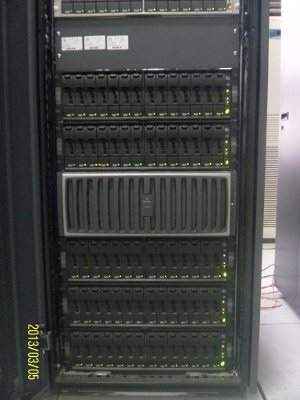
\includegraphics{raiddisk}
%   \caption{磁盘阵列}
%   \label{fig:xfig9}
% \end{figure}

\section{文档的撰写与展示}
\label{sec:writeandview}

本系统鼓励用户使用\smarkdown在系统内直接撰写文档,但是考虑到用户的使用习惯不会在段时间内改变,所以系统在用户文档的设计部分,充分考虑到了word用户可以轻松上手的功能,首先系统提供了和Word操作很相似的富文本编辑页面与\smarkdown互为补充,用户可以按照自己的喜好选择自己喜欢的编辑环境。其次系统还提供了Word等格式文档的上传与预览功能。以满足Word用户的需要。

上文中曾经批评过Windows操作系统的文档管理中目录结构松散,与缺乏标签管理等问题。那么,本系统中的文档组织又是什么样的呢? 如%图~\ref{fig:xfig10}
所示,显然,本系统的文档组织也是由目录组成。但是这里的目录的概念和window操作系统中的目录概念不太一样。本系统的文档组织有如下特点:
\begin{enumerate}
\item 每一篇文档都隶属一个目录。
\item 每篇文档都由文档内容和若干文档属性组成,在编辑文档内容的时候,可以插入文档属性到内容中。文档显示的时候,插入的文档属性可以以用户选取的方式显示在文档中。文档的
\end{enumerate}
下面简单说明一下系统提供哪些类型的文档属性